\documentclass[class=book, crop=false, oneside]{standalone}
\usepackage[subpreambles=true]{standalone}

\usepackage{../../style}
\usepackage{../../set-citations}

\graphicspath{{./assets/images/}}

% arara: pdflatex: { synctex: yes, shell: yes }
% arara: latexmk: { clean: partial }
\begin{document}
\chapter{La gerarchia di memoria}\begin{fquote}[Burks, Goldstine, Von Neumann][1946]Idealmente si desidererebbe una memoria indefinitamente grande, in cui ogni particolare parola risulti immediatamente disponibile.
 \end{fquote}

\section{Introduzione}
Sottolineare quanto il concetto di memoria sia importante e necessario nei dispositivi elettronici del giorno d'oggi risulta abbastanza scontato. D'altra parte, viene fatta subito una precisazione: non esiste un'unica soluzione che permette di ottenere la memoria "perfetta". Esistono infatti diverse implementazioni, ognuna con i suoi compromessi, che variano per costo, prestazioni e capacità.

\section*{Qualche definizione}
Possiamo distinguere principalmente due tipologie di memoria in base alla modalità di accesso:
\begin{itemize}
	\item \emph{memoria indirizzata direttamente} (memoria principale, memoria cache):
	\begin{itemize}
		\item è volatile, ossia il suo contenuto viene perso se viene spento il calcolatore;
		\item è limitata per capacità dallo spazio di indirizzamento definito dall'architettura del processore;
		\item i dati contenuti nella memoria principale sono disponibili in qualsiasi momento;
	\end{itemize}
	\item \emph{memoria indirizzata indirettamente} (memoria periferica):
	\begin{itemize}
		\item è di tipo permanente, ossia mantiene il suo contenuto anche senza alimentazione;
		\item ha uno spazio di indirizzamento software che non dipende dall'architettura del processore;
		\item i dati contenuti nella memoria periferica devono essere trasferiti alla memoria principale prima di essere utilizzati (solitamente questo processo viene mediato dal software, tipicamente il sistema operativo);
	\end{itemize}
\end{itemize}

A seguire un elenco di definizioni che utilizzeremo in seguito:
\begin{itemize}
	\item \emph{Tempo di accesso}: è il tempo richiesto per \emph{una} operazione di lettura / scrittura nella memoria;
	\item \emph{Tempo di ciclo}: è il tempo che intercorre fra l'inizio di due istruzioni consecutive; è composto dal tempo di accesso sommato al tempo per muovere il dato con cui si stava lavorando;
	\item \emph{Accesso casuale}: è quella modalità di accesso in cui non vi è alcun ordine o relazione fra i dati memorizzati; è tipico delle memorie a semiconduttori;
	\item \emph{Accesso sequenziale}: è quella modalità che presuppone lo scorrimento ordinato di un blocco di dati per accere ad un suo dato; il tempo d'accesso dipende dalla posizione fisica del dato nel supporto (tipicamente nastri e dischi);
	\item \emph{RAM} (\emph{Random Access Memory}): è una memoria dotata di accesso casuale che permette scrittura e lettura; viene implementata attraverso semiconduttori;
	\item \emph{ROM} (\emph{Read Only Memory}): è una memoria a semiconduttori che prevede solo un accesso in lettura; esistono implementazioni sia attraverso accesso casuale che sequenziale
\end{itemize}

\section{La memoria principale}
\subsection{Le RAM}
Con la seguente immagine descriviamo come avviene la connessione logica fra memoria RAM e CPU:
\begin{figure}[H]
	\centering
	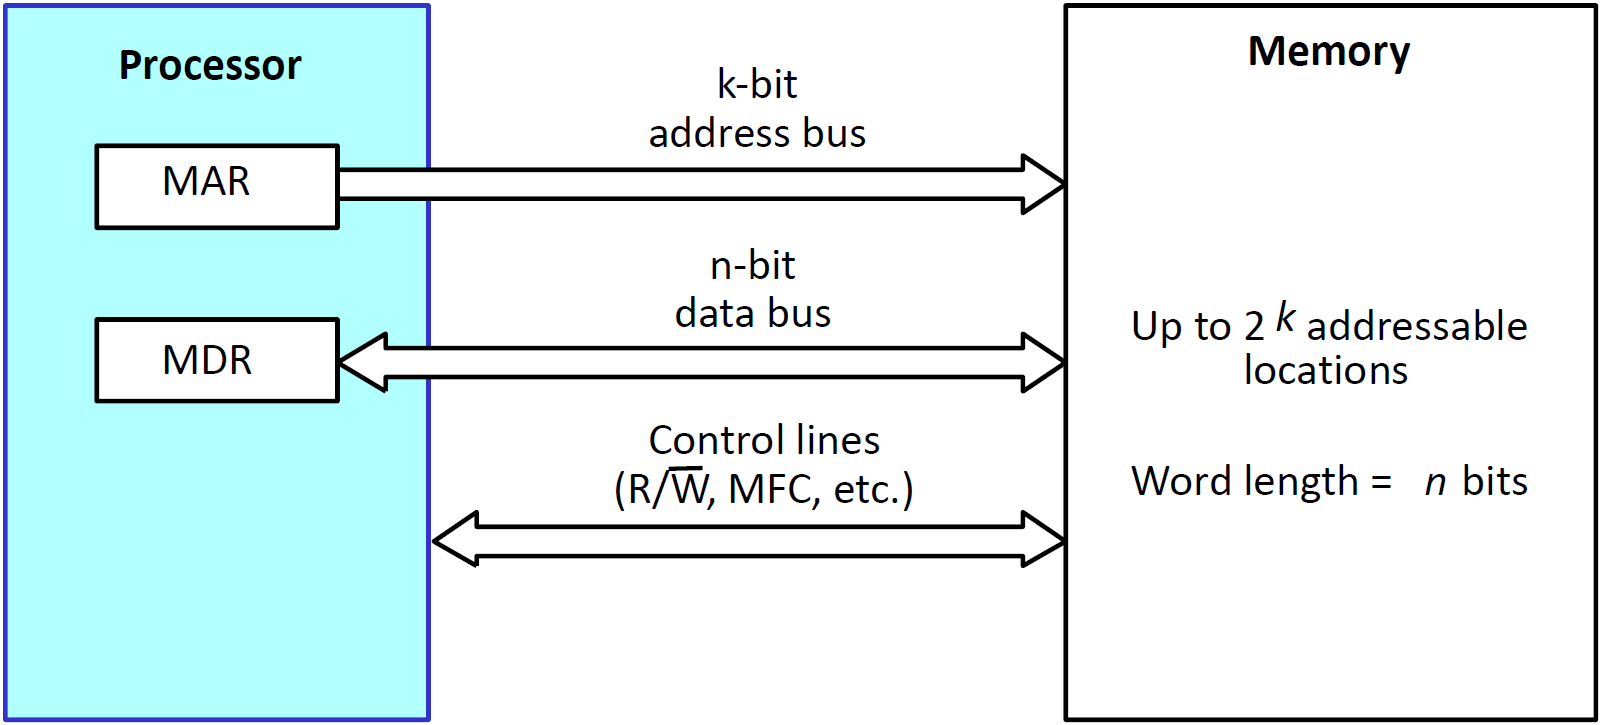
\includegraphics[width=\textwidth,keepaspectratio]{relazione_cpu_ram.png}
	\caption{Modello della relazioni logiche fra CPU e RAM}
\end{figure}
Esistono principalmente 3 bus che permettono di far comunicare il processore con la memoria:
\begin{itemize}
	\item \emph{MAR} (\emph{Memory Address Register}): è un bus a \(k\) bit, dove \(2^k\) sono il numero massimo di indirizzi accessibili direttamente in memoria. Dal punto di vista pratico contiene l'indirizzo del dato (o istruzione) che si vuole caricare o scrivere;
	\item \emph{MDR} (\emph{Memory Data Register}): è un bus a \(n\) bit, dove \(n\) è la lunghezza delle word nella memoria. Dal punto di vista pratico contiene il dato (o l'istruzione) che si vuole caricare o scrivere;
	\item \emph{bus di controllo:} è un bus che contiene vari codici di controllo che permettono di pilotare le relazioni fra memoria e CPU. Alcune linee di controllo sono: il bit \emph{MFC} (\emph{Memory Function Completed}) che permette di stabilire se l'operazione di lettura o scrittura è stata completata e il bit \emph{\(\textrm{R/}\overline{W}\)}, che distingue se si sta eseguendo un'operazione di lettura o scrittura.
\end{itemize}
Si noti che il \emph{MAR} è stato rappresentato da una freccia unidirezionale: dopo aver definito l'indirizzo di memoria su cui lavorare, infatti il processore non si aspetta il risultato. Vengono gestiti diversamente i bus di controllo e \emph{MDR}, i quali sono rappresentati con una freccia bidirezionale, in quanto sia la memoria che la CPU possono occupare il ruolo di mittente del messaggio.

Una memoria \emph{RAM} a semiconduttori principalmente memorizza singoli bit, memorizzati normalmente in gruppi di byte e/o word per motivi di efficienza. La memoria non necessariamente deve essere strutturata singolarmente: è possibile che sia suddivisa in diversi blocchi, al fine di favorire il parallelismo (si noti comunque che la dimensione complessiva della memoria non varia se presa in un unico blocco o se separata. Si ricorda che l'organizzazione di una memoria influenza il numero di pin di I/O del circuito integrato: più saranno, più aumenterà il costo.

\subsubsection{Organizzazione dei bit in un banco di memoria 16x8}
\begin{figure}[H]
	\centering
	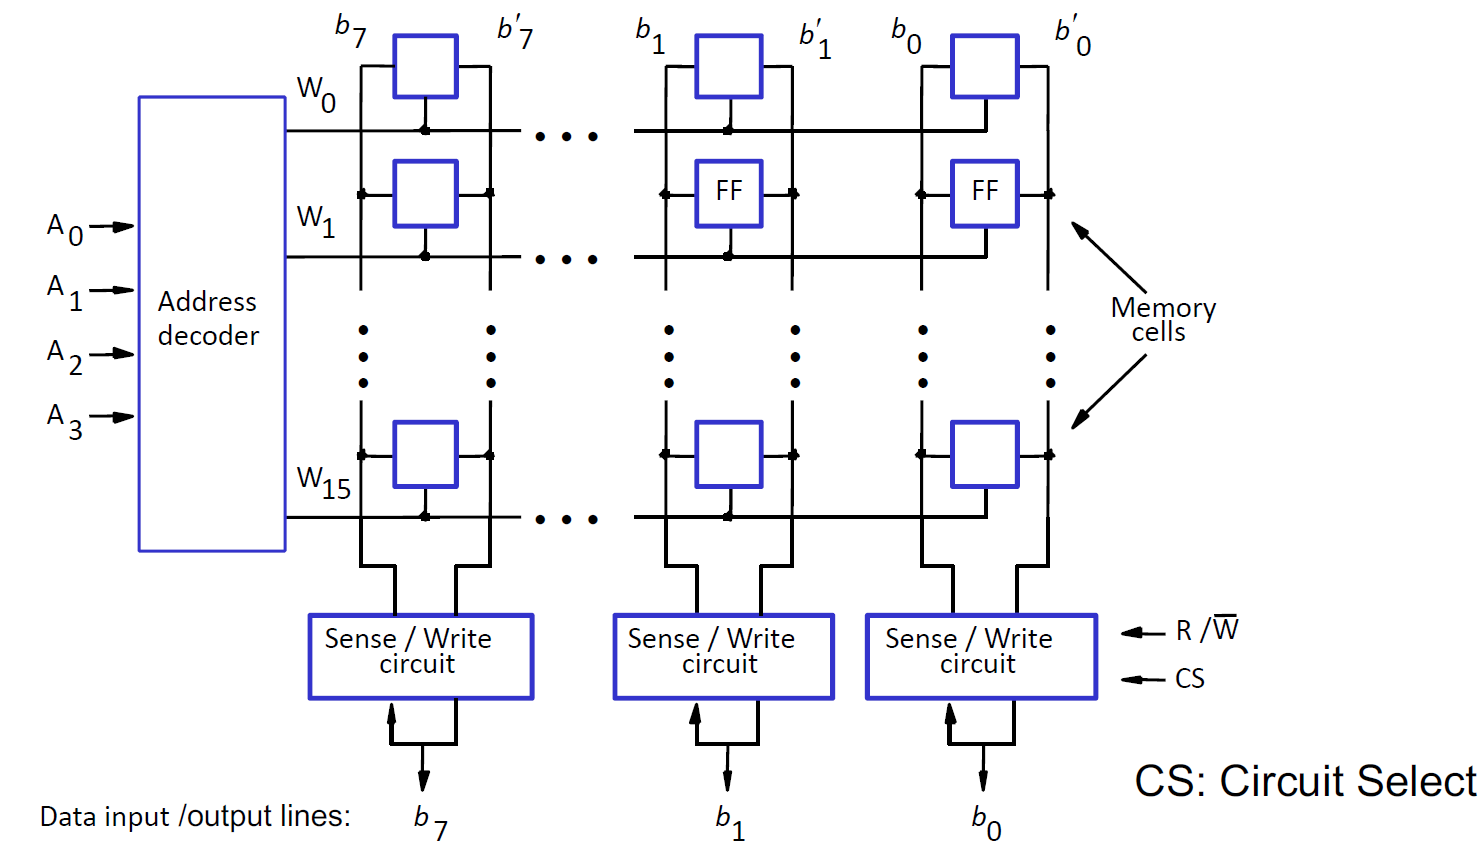
\includegraphics[width=\textwidth,keepaspectratio]{organizzazione.png}
	\caption{Organizzazione di un banco di memoria 16x8}
\end{figure}
Il caso presentato descrive il funzionamento di un banco di memoria formato da 16 righe e 8 colonne, con celle da un byte ciascuna. Si noti che per indirizzare un certo elemento all'interno della matrice del banco di memoria è necessario attivare una determinata riga e colonna (come avverrebbe in battaglia navale). Analizziamo ora, in ordine temporale, le operazioni che permettono di accedere/scrivere un determinato dato.
\begin{enumerate}
	\item In base alla riga da selezionare, l'\emph{address decoder} genera un 1 nell'uscita della riga corrispondente;
	\item Avviene un meccanismo simile anche per le colonne, attraverso il \emph{circuit select}, che decide se abilitare ciascuna colonna;
	\item Ogni colonna è gestita da un \emph{Sense/Write circuit} che riceve in input due linee di controllo: una definisce se eseguire l'operazione di lettura o scrittura (\emph{\(\textrm{R/}\overline{W}\)}) mentre l'altra (\emph{CS}) definisce se attivare o meno la colonna. Nel caso di una read, legge il valore contenuto nel bus della colonna (1 byte nel nostro esempio), altrimenti, nel caso di write, fa circolare il valore che si vuole scrivere nel bus della colonna. Per avere certezza dell'integrità dei dati, viene propagato sia il dato stesso che si vuole scrivere, che il suo negato. Ad esempio, nella colonna 0, \(b_0\) contiene il dato asserito, mentre \(b'_0\) contiene il dato negato;
	\item In base a com'è stata implementata la memoria (\emph{SRAM} o \emph{DRAM}), viene attivata la cella selezionata dalla colonna e dalla riga designata: su di essa verrà eseguita l'operazione di lettura/scrittura richiesta.
\end{enumerate}

Nelle prossime sezioni affronteremo come varia l'implementazione di ciascuna cella di memoria da \emph{SRAM} a \emph{DRAM}.

\subsection{Le SRAM}
Le \emph{SRAM}, ossia le RAM statiche, sono delle memorie in cui i bit possono essere mantenuti indefinitivamente (posto il fatto che non manchi l'alimentazione). Seppur abbiano tempi di accesso molto ridotti (nell'ordine di pochi nanosecondi) e consumino poca corrente, il loro costo è molto elevato: per ciascuna cella di memorizzazione vengono impiegati molteplici componenti.
Il funzionamento che sta alla base di una cella di SRAM è quello del flip flop (in particolare ai latch tipo D).

\subsection{Le DRAM}







\end{document}
